% ------------------------------------------------------------------------------
% TYPO3 CMS 7.0 - What's New - Chapter "Deprecated Functions" (English Version)
%
% @author	Michael Schams <schams.net>
% @license	Creative Commons BY-NC-SA 3.0
% @link		http://typo3.org/download/release-notes/whats-new/
% @language	English
% ------------------------------------------------------------------------------
% LTXE-CHAPTER-UID:		1a0c6db9-8f24051e-f9c8847a-d7e05fd2
% LTXE-CHAPTER-NAME:	Deprecated Functions
% ------------------------------------------------------------------------------

\section{Verouderde/verwijderde functies}
\begin{frame}[fragile]
	\frametitle{Verouderde/verwijderde functies}

	\begin{center}\huge{Hoofdstuk 5:}\end{center}
	\begin{center}\huge{\color{typo3darkgrey}\textbf{Verouderde/verwijderde functies}}\end{center}

\end{frame}

% ------------------------------------------------------------------------------
% LTXE-SLIDE-START
% LTXE-SLIDE-UID:		6427462e-5359504c-34340003-2f29c751
% LTXE-SLIDE-ORIGIN:	c47248f9-03aa1da2-8dd9985d-762cf405 English
% LTXE-SLIDE-TITLE:		Legacy Layer
% LTXE-SLIDE-REFERENCE:	http://typo3.org/news/article/retaining-compatibility-to-typo3-cms6/
% ------------------------------------------------------------------------------

\begin{frame}[fragile]
	\frametitle{Verouderde/verwijderde functies}
	\framesubtitle{Compatibiliteitslaag}

	\begin{itemize}

		\item TYPO3 CMS 6.2: een compatibliteitslaag zorgt ervoor dat oude extensies werken in de nieuwe code\newline
			\small
				Nadeel: verminderde prestaties (niet het volledige potentieel van het systeem)
			\normalsize

		\item TYPO3 CMS 7.0: compatibiliteitslaag is verwijderd uit de core\newline
			\small
				Impact: oude extensies werken mogelijk niet (bijv. extensies zonder namespaces)
			\normalsize

		\item Compatibiliteit kan indien nodig toegevoegd worden via de systeemextensie \texttt{EXT:compatibility6}
		\item Deze extensie wordt in de toekomst naar de TER verhuisd

	\end{itemize}

\end{frame}

% ------------------------------------------------------------------------------
% LTXE-SLIDE-START
% LTXE-SLIDE-UID:		36fc5525-dbfc42e3-b777e658-d6622df2
% LTXE-SLIDE-ORIGIN:	70da8aab-cd42e15f-fe254b81-41ceabb5 English
% LTXE-SLIDE-TITLE:		Backend User Management
% ------------------------------------------------------------------------------

\begin{frame}[fragile]
	\frametitle{Verouderde/verwijderde functies}
	\framesubtitle{Beheer van backendgebruikers}

	\begin{itemize}
		\item Overschakelen naar backendgebruiker ("wissel-naar-modus") is verwijderd
	\end{itemize}

	\smaller\tabto{1cm}\begingroup\color{typo3red}TYPO3 CMS 6.2\endgroup\normalsize
	\begin{figure}\vspace{-0.4cm}
		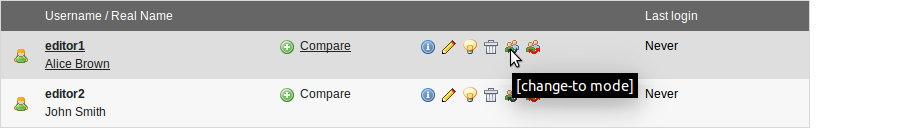
\includegraphics[width=0.90\linewidth]{DeprecatedRemovedFunctions/BackendUserSwitch1.png}
	\end{figure}

	\smaller\tabto{1cm}\begingroup\color{typo3red}TYPO3 CMS 7.0\endgroup\normalsize
	\begin{figure}\vspace{-0.4cm}
		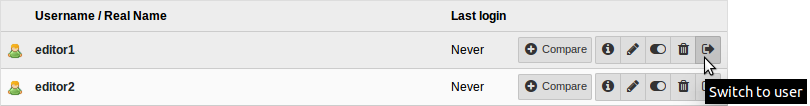
\includegraphics[width=0.90\linewidth]{DeprecatedRemovedFunctions/BackendUserSwitch2.png}
	\end{figure}

\end{frame}

% ------------------------------------------------------------------------------
% LTXE-SLIDE-START
% LTXE-SLIDE-UID:		1e6e09cc-55502ea2-4371e411-f47e5f4e
% LTXE-SLIDE-ORIGIN:	10805d4d-787ce2f8-10e4329a-1451521a English
% LTXE-SLIDE-TITLE:		Removed Deprecated JavaScript Functions
% LTXE-SLIDE-REFERENCE:	https://github.com/TYPO3/TYPO3.CMS/commit/2dff81b963e1b77c7f068f91ffde73914a18b0be
% LTXE-SLIDE-REFERENCE:	https://forge.typo3.org/issues/62291
% LTXE-SLIDE-REFERENCE:	https://forge.typo3.org/projects/typo3cms-core/repository/revisions/9ac03e383e4786e868f4b1d81893e84c4621abc8/entry/typo3/sysext/core/Documentation/Changelog/master/Breaking-62291-RTEDeprecatedJavaScriptMethodsRemoved.rst
% ------------------------------------------------------------------------------

\begin{frame}[fragile]
	\frametitle{Verouderde/verwijderde functies}
	\framesubtitle{Verouderde Javascript-functies verwijderd}

	\begin{itemize}
		\item Conform de \href{http://forge.typo3.org/projects/typo3v4-core/wiki/CoreDevPolicy}{verouderingsstrategie}
			zijn een aantal JavaScript-methodes verwijderd die sinds TYPO3 CMS 4.7 als \textit{verouderd} waren aangemerkt:

		\begin{lstlisting}
			\TYPO3\CMS\Backend\Form\FormEngine->getSingleField_typeInput
			\TYPO3\CMS\Backend\Form\FormEngine->getSingleField_typeText
			\TYPO3\CMS\Core\Utility\GeneralUtility->quoted_printable
			\TYPO3\CMS\Core\Utility\GeneralUtility->encodeHeader
		\end{lstlisting}

		\smaller
			\texttt{HTMLArea.Editor.forceRedraw}\newline
				(gebruik in plaats hiervan \texttt{HTMLArea.Framework.doLayout})
				\vspace{0.2cm}

			\texttt{HTMLArea.Editor.convertNode}\newline
				(gebruik in plaats hiervan \texttt{HTMLArea.DOM.convertNode})
				\vspace{0.2cm}

			\texttt{HTMLArea.Editor.getBlockAncestors}\newline
				(gebruik in plaats hiervan \texttt{HTMLArea.DOM.getBlockAncestors})
		\normalsize

	\end{itemize}

\end{frame}

% ------------------------------------------------------------------------------
% LTXE-SLIDE-START
% LTXE-SLIDE-UID:		f5db0561-94977747-c49d8bcb-12de2f66
% LTXE-SLIDE-ORIGIN:	9da41efc-970e66a8-f9163c40-67cfa712 English
% LTXE-SLIDE-TITLE:		Removed Functions (1)
% LTXE-SLIDE-REFERENCE:	https://forge.typo3.org/issues/17579
% LTXE-SLIDE-REFERENCE:	https://forge.typo3.org/issues/62888
% ------------------------------------------------------------------------------

\begin{frame}[fragile]
	\frametitle{Verouderde/verwijderde functies}
	\framesubtitle{Verwijderde functies (1)}

	\begin{itemize}

		\item
			\small
				TypoScript-instelling \texttt{config.uniqueLinkVars} is verwijderd\newline
				(dit gedrag is nu standaard)
			\normalsize

		\item
			\small
				ViewHelper
					\texttt{\textbackslash
						TYPO3\textbackslash
						CMS\textbackslash
						Documentation\textbackslash
						ViewHelpers\textbackslash
						Link\textbackslash
						Action}
					is verwijderd (gebruik \texttt{f:be.buttons.icon} of \texttt{f:uri.*} in plaats hiervan)
			\normalsize

		\item
			\small
				PageTSconfig-optie \texttt{mod.web\_list.alternateBgColors}\newline
				is verwijderd
			\normalsize

		\item
			\small
				PropertyMapper is verwijderd\newline
				(inclusief optie \texttt{rewrittenPropertyMapper = 0})
			\normalsize

		\item
			\small
				TypoScript-condities zijn verwijderd:

					\begin{itemize}
						\item\texttt{browser}
						\item\texttt{version}
						\item\texttt{system}
						\item\texttt{useragent}
					\end{itemize}
			\normalsize

	\end{itemize}

\end{frame}

% ------------------------------------------------------------------------------
% LTXE-SLIDE-START
% LTXE-SLIDE-UID:		8ff3d1d6-c23a32b5-59b90634-ca2aa3f4
% LTXE-SLIDE-ORIGIN:	efe86631-b6020ae8-ffa01160-6de29dc3 English
% LTXE-SLIDE-TITLE:		Removed Functions (1)
% ------------------------------------------------------------------------------

\begin{frame}[fragile]
	\frametitle{Verouderde/verwijderde functies}
	\framesubtitle{Verwijderde methodes (1)}

	De volgende \textbf{methodes} zijn verwijderd:

	\begin{itemize}
		\item
			\small
				\texttt{connectDB}\newline
				van klasse
				\texttt{\textbackslash
					TYPO3\textbackslash
					CMS\textbackslash
					Frontend\textbackslash
					Utility\textbackslash
					EidUtility}
			\normalsize
		\item
			\small
				\texttt{isDisplayCondition}\newline
				van klasse
				\texttt{\textbackslash
					TYPO3\textbackslash
					CMS\textbackslash
					Form\textbackslash
					FormEngine}
			\normalsize
		\item
			\small
				\texttt{int\_from\_ver}\newline
				van klasse
				\texttt{\textbackslash
					TYPO3\textbackslash
					CMS\textbackslash
					Core\textbackslash
					Utility\textbackslash
					GeneralUtility}
			\normalsize
		\item
			\small
				\texttt{getUniqueFields}\newline
				van klasse
				\texttt{\textbackslash
					TYPO3\textbackslash
					CMS\textbackslash
					Core\textbackslash
					DataHandling\textbackslash
					DataHandler}
			\normalsize

	\end{itemize}

\end{frame}

% ------------------------------------------------------------------------------
% LTXE-SLIDE-START
% LTXE-SLIDE-UID:		aff427e7-1556ef4c-e3118e24-aabf1955
% LTXE-SLIDE-ORIGIN:	293414d4-e87db3d5-afced471-ca9826ed English
% LTXE-SLIDE-TITLE:		Removed Methods (2)
% ------------------------------------------------------------------------------

\begin{frame}[fragile]
	\frametitle{Verouderde/verwijderde functies}
	\framesubtitle{Verwijderde Methodes (2)}

	De volgende \textbf{methodes} zijn verwijderd:

	\begin{itemize}

		\item
			\small
				\texttt{isSafeModeEnabled}\newline
				van klasse
				\texttt{\textbackslash
					TYPO3\textbackslash
					CMS\textbackslash
					Core\textbackslash
					Utility\textbackslash
					PhpOptionsUtility}
			\normalsize
		\item
			\small
				\texttt{registerSwiftMailer}\newline
				van klasse
				\texttt{\textbackslash
					TYPO3\textbackslash
					CMS\textbackslash
					Core\textbackslash
					Bootstrap}
			\normalsize
		\item
			\small
				\texttt{loadTCA}\newline
				van klasse
				\texttt{\textbackslash
					TYPO3\textbackslash
					CMS\textbackslash
					Core\textbackslash
					Utility\textbackslash
					GeneralUtility}
			\normalsize
		\item
			\small
				\texttt{isLocalconfWritable}\newline
				van klasse
				\texttt{\textbackslash
					TYPO3\textbackslash
					CMS\textbackslash
					Core\textbackslash
					Utility\textbackslash
					ExtensionManagementUtility}
			\normalsize

	\end{itemize}

\end{frame}

% ------------------------------------------------------------------------------
% LTXE-SLIDE-START
% LTXE-SLIDE-UID:		81f132a1-c003fb53-48666c69-3e9625e1
% LTXE-SLIDE-ORIGIN:	a1ba1998-f88c1063-71470741-30b9f314 English
% LTXE-SLIDE-TITLE:		Removed Classes
% ------------------------------------------------------------------------------

\begin{frame}[fragile]
	\frametitle{Verouderde/verwijderde functies}
	\framesubtitle{Verwijderde Klassen}

	De volgende \textbf{klassen} zijn verwijderd:

	\begin{itemize}

		\item
			\smaller
				\texttt{\textbackslash
					TYPO3\textbackslash
					CMS\textbackslash
					Backend\textbackslash
					Template\textbackslash
					MediumDocumentTemplate}
			\normalsize
		\item
			\smaller
				\texttt{\textbackslash
					TYPO3\textbackslash
					CMS\textbackslash
					Extbase\textbackslash
					Service\textbackslash
					TypeHandlingService}
			\normalsize

	\end{itemize}

\end{frame}

% ------------------------------------------------------------------------------
